To learn how cooperative behaviors may influence success ratio in a particular task, the decision was made to first observe the evolution in case where agents work against one another, competing for a higher score. Only then, comparing the results with those of a cooperative case, conclusions regarding cooperation influence may be drawn.

The scenarios were tested in parallel with each change, were it to complicate the problem or put emphasis on certain components of the solutions.

The two scenarios shall be described in their dedicated sections below, focusing on key contrast points. Following, however, are the elements common to both cases.

Evaluation process of candidate solutions was made in the same environment, with identical starting points and resource markers' locations. In both scenarios, trees produced by Genetic Programming are accompanied by a unchanging, user-defined tree in the simulations. This reference agent uses one type of Action, \textit{goToFlag(flagNumber)}, visiting each resource marker in turn, capturing them from first to last, never changing path between simulations. Figure \ref{fig:x referenceagentdiagram} presents the Behavior Tree schematic of the reference agent. Existence of such tree could fill the function of both a pressuring component (reflected in the fitness function in the appropriate cases) and essentialy a time-gate, as gathering all markers would end the simulation. Furthermore, algorithms in both cases had access to identical Behavior Tree Components to build the trees from, thus ensuring equal sophistication of solutions in each scenario.

\begin{figure}[h]
    \centering
    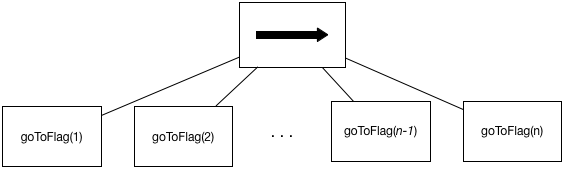
\includegraphics[scale=0.4]{referenceagentdiagram}
    \caption{A schematic of reference agent used in simulations.}
    \label{fig:x referenceagentdiagram}
\end{figure}
\section{Competitive Scenario Specification}
\subsection{Synopsis}
Competitive case assumed the optimal solution to the problem is maximizing the agent's personal gain. The markers gathered were counted for each agent separately, thus turning the task into a race - evolutionary agent was forced to get to as many markers as possible before the reference agent would claim them for himself.

After initial testing, the scenario was modified to feature 7 resource markers (instead of initial 5) and modified spawn points of agents -  readjusted to move evolutionary agent further back from the first marker. While increasing the number of markers served as an attempt to complicate the problem, moving evolutionary agent further from the first flag was done in the interest of being able to reproduce the results: since both agents were in the equal distance of the first flag and moved with the same speed, the matter of which one would claim the first flag was comparable to a coin-toss. Figure \ref{fig:x scenario1topdown} presents the final view of the competitive scenario map.

\begin{figure}[h]
    \centering
    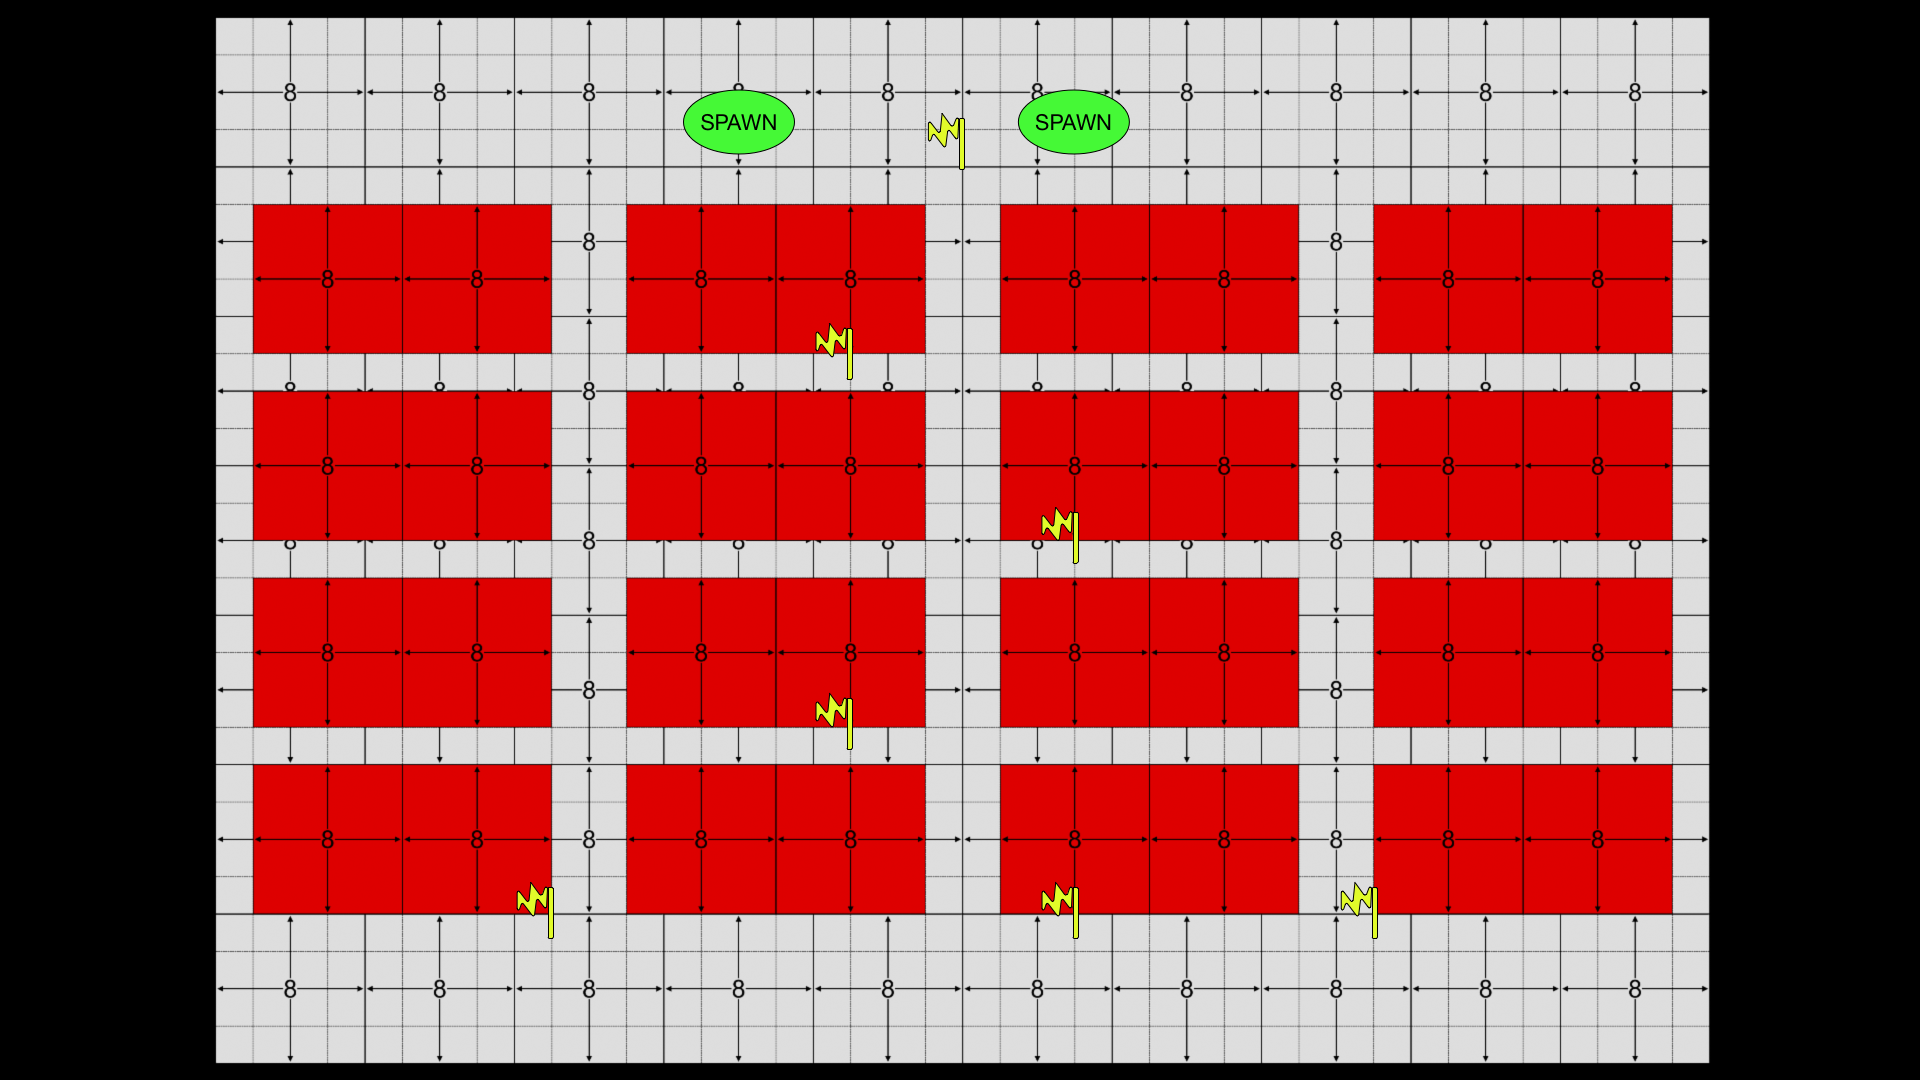
\includegraphics[scale=0.2]{scenario1topdown}
    \caption{Finished map of the competitive scenario environment}
    \label{fig:x scenario1topdown}
\end{figure}

\subsection{Fitness Function}
The competitive scenario is effectively a zero-sum game: a gain in utility of one agent means (prospective) loss of utility for the others. Considering that, the initial fitness value of the $i-th$ specimen in the population was a sum of $n$ markers gathered by an agent controlled by a tested tree, multiplied by a resource point constant $C_1$. This, however, wasn't feasible as a long-term solution. To introduce differentiability between the specimen scoring the same amounts of markers, a  factor of time in milliseconds multiplied by constant $C_2$ was then subtracted from the sum. Additionally, to coerce the algorithm into preferring smaller trees, a tree size factor with weight $C_3$ was further subtracted from this value. The finished formula for fitness function is presented on Equation \ref{eq:x scenario1fitness}.
\begin{equation}
    \label{eq:x scenario1fitness}
f(i) = C_1 * n - (\frac{t}{C_2} + \frac{s}{C_3})
\end{equation}
\subsection{Success Criterion}
\label{section_competitive_success}
With the goal of maximizing personal gain, which is the case with the considered scenario, desirable trees are those that claim every possible marker. However, since evolutionary agent's spawn position put it at the disadvantage (making it impossible to gather the first flag), only solutions with $n - 1$ flags gathered out of $n$ possible would be considered ``successful''. The true goal of a ideal solution was then to create a big enough difference in time taken to visit the markers, allowing it to reach and claim the last one.
\section{Cooperative Scenario Specification}
\subsection{Synopsis}
Cooperative scenario, in contrast to the ``selfishly'' motivated competitive one, takes a broader perspective. Instead of competing, agents were expected to work with each other towards claiming all 5 markers. However in time, the layout of the scenario was modified to maintain uniformity between the two cases' layout - that included both increasing the number of flags to 7 and modifying the agents' spawn positions - for comparison reasons.
\subsection{Fitness Function}
Due to competitive aspect being gone, a perspective on performance shifted substantially. The number of markers claimed by an agent became an impractical characteristic, with the time factor providing a much more considerable view on specimen performance. However, the decision was made to include the \textit{total number of markers} in the fitness function, serving as a constant, to ensure that the results from both scenarios are of the same order of magnitude. Aforementioned time and tree size components remained in untouched form, all the more critical in case at hand. Equation \ref{eq:x scenario2fitness} presents the fitness function used in evaluating specimen in cooperative scenario.
\begin{equation}
    \label{eq:x scenario2fitness}
f(i) = C_1 * (n + m) - (\frac{t}{C_2} + \frac{s}{C_3})
\end{equation} % legend?

\subsection{Success Criterion}
\label{section_cooperative_success}
In the cooperative case, the underlaying goal is to divide the markers between two agents in the most efficient way. To effectively operate, the desired outcome is achieving completion time shorter than the time it takes for the reference agent to complete his route. In other words, a successful solution will be able to successfully adapt itself to a potential partner's route and improve upon it in terms of time.

\section{Fitness Function Parameters}
\label{section_fitness_function_tuning}
The aforementioned point constants of the fitness function, defined as follows:
\begin{itemize}
    \item $C_1$ - resource marker point value
    \item $C_2$ - time factor weight
    \item $C_3$ - tree size weight
\end{itemize}
Were tuned by using \textit{grid-search} algorithm with a number of possible values of $C_2$ and $C_3$. $C_1$, however, remained unchanged. The decision was made that, for the purposes of the competitive case, the number of resource markers should remain the deciding factor.
The values of the parameters after grid-search tuning are presented in tables \ref{table:x tunedfitnessfunctionparameterscoop} and \ref{table:x tunedfitnessfunctionparameterscomp}.
\begin{table} [h]
    \centering
    \begin{tabular} {l r}
        \hline \hline
        Parameter Name & Parameter Value \\
        \hline
        $C_1$ - resource marker point value & 1000 \\
        $C_2$ - time factor weight & 0.1 \\
        $C_3$ - tree size weight & 100 \\
    \end{tabular}
    \caption{Selected Fitness Function factor weights for Cooperative Scenario}
    \label{table:x tunedfitnessfunctionparameterscoop}
\end{table}


\begin{table} [h]
    \centering
    \begin{tabular} {l r}
        \hline \hline
        Parameter Name & Parameter Value \\
        \hline
        $C_1$ - resource marker point value & 1000 \\
        $C_2$ - time factor weight & 0.01 \\
        $C_3$ - tree size weight & 10 \\
    \end{tabular}
    \caption{Selected Fitness Function factor weights for Competitive Scenario}
    \label{table:x tunedfitnessfunctionparameterscomp}
\end{table}
\section{Genetic Programming Parameters in Experiments}
After observing the results from a number of initial test runs as well as using \textit{grid-search} algorithm to help determine \textit{crossover rate}, \textit{mutation rate} and \textit{population size} parameters, the parameters used in the experiments are presented in table \ref{table:x selectedgpparameters}.

\begin{table} [h]
    \centering
    \begin{tabular} {l r}
        \hline \hline
        Parameter Name & Parameter Value \\
        \hline
        Maximum Number of Generations & 100 \\
        Population Size & 200 \\
        Crossover Rate & 25\% \\
        Micromutation Rate & 15\% \\
        Macromutation Rate & 2\% \\
        Tournament Selection Tourney Size & 10 \\
    \end{tabular}
    \caption{Selected Genetic Programming parameter values.}
    \label{table:x selectedgpparameters}
\end{table}

After a number initial runs, it was clear that keeping a maximum number of generations above one hundred served no function - there were no instances that did not converge before that point and following were long periods of stagnation or, even worse, loosing best specimen. The method responded positively to increasingly higher number of specimen in the generation: totaling at 200, this ensures a good variety of genetic material for the algorithm to make use of. Crossover and mutation rates were kept low due to the risk of destroying relatively low number of good specimen each generation. On the other hand, they could not have been set \textit{too low}, lest the algorithm would not explore the search space properly. It is worth pointing out that macromutation (``Headless Chicken'') was kept at extremely low occurrence chance specifically for that reason - there weren't any instances suffering from too early convergence, something that macromutation would have been a remedy to. Choosing a 5\% value of tourney size ensured it would still be possible to get specimen with mid-range fitness value into the next generation while keeping the selection pressure relatively high.

Table \ref{table:x selectedbtparameters} presents selected parameters used during tree generation steps in the algorithm.
\begin{table} [h]
    \centering
    \begin{tabular} {l r}
        \hline \hline
        Parameter Name & Parameter Value \\
        \hline
        Maximum Tree Depth & 6 \\
        Starting Generation Minimum Tree Size & 20 \\
        Starting Generation Maximum Tree Size & 30 \\
        Headless Chicken Generated Tree Minimum Size & 10 \\
        Headless Chicken Generated Tree Maximum Size & 20 \\
        Headless Chicken Maximum Tree Depth & 5 \\
        Expected \textit{Action-to-Composite} node Ratio & 3:1 \\
    \end{tabular}
    \caption{Selected Behavior Tree generation parameter values.}
    \label{table:x selectedbtparameters}
\end{table}
The tree related parameters were chosen after a careful consideration of desirable feats both in the initial generation as well as during rarely-observed macromutation. Generating the tree between 20 and 30 nodes would create a varied populations with different shaped trees, while maintaining decent complexity bound by maximum tree depth. The need for larger number of Actions in relation to Composite nodes was dictated by a simplicity of the task and in the interest of further coercing the algorithm to prefer simpler structures.
\newpage
\section{Exemplary Specimen}
In this section, a sample specimen representation is presented and described. The listing below presents the text representation of a tree, while figure \ref{fig:x exemplaryspecimenscenario1} contains a (arguably) more human-readable form.
\begin{lstlisting}
Sequence
  ActionGoToFlag 0
  ActionGoToFlag 3
  ActionGoToFlag 4
  ActionGoToFlag 4
  Selector
    Sequence
      Selector
        Sequence
          ActionGoToFlag 7
          ActionGoToFlag 5
          ActionGoToFlag 6
        ActionGoToFlag 6
      ActionGoToFlag 0
      ActionGoToFlag 3
      ActionGoToFlag 4
    ActionGoToFlag 3
    ActionGoToFlag 7
  Sequence
    ActionGoToFlag 2
    ActionGoToFlag 3
  ActionGoToFlag 4
  Selector
    ActionGoToFlag 1
    ActionGoToFlag 1
  ActionGoToFlag 5
  ActionGoToFlag 2
  ActionGoToFlag 3
\end{lstlisting}

\begin{figure}[h]
    \centering
    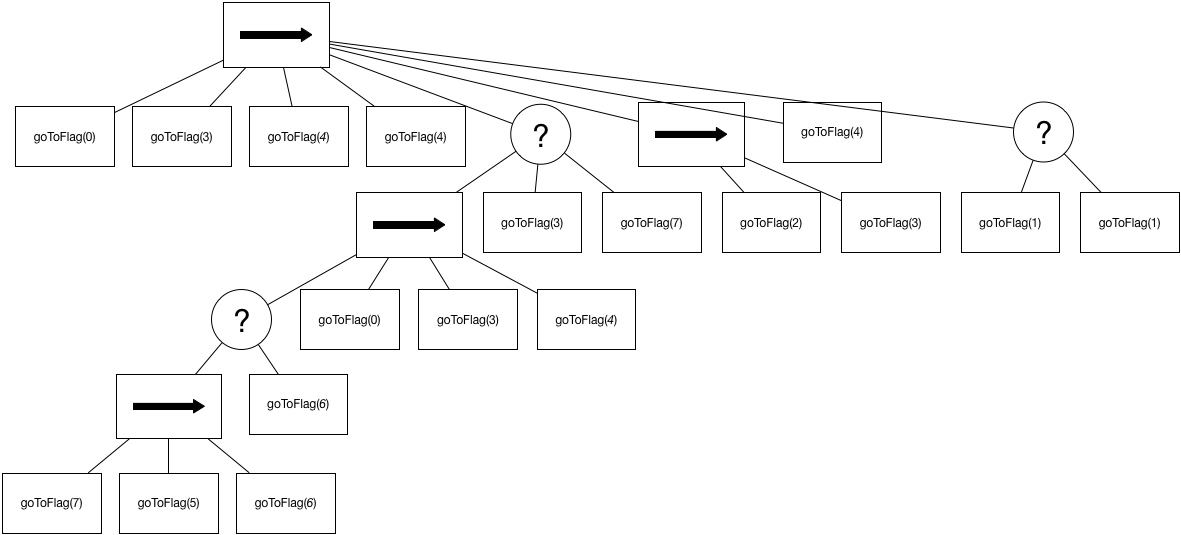
\includegraphics[scale=0.4]{exemplaryspecimenscenario1}
    \caption{Example diagram of a evolutionary generated specimen.}
    \label{fig:x exemplaryspecimenscenario1}
\end{figure}

This particular specimen was generated during one of competitive scenario experiments and his evaluation placed it on value 5911. Knowing both the value of fitness value constants it can be proven that the specimen claimed 6 resource markers out of 7 possible.

The tree has a very cluttered look and many unnecessary placed nodes, but the route should be clear: going from the top, it's going to visit the closest marker, which is the second one (sic!), then the third, proceeding to the fourth one (twice, in fact, but the second call will return instantly) and head for the last one, only to return to the fifth and sixth, probably meeting a reference agent nearby fifth marker. The rest of the nodes, as mentioned before, serve no function in this particular scenario. Unfortunately, the tree didn't follow the expected strategy (gaining a bit on each marker only to make a final push from sixth to seventh) instead opting to devise a new one. Although - as seen above - the strategy of choice seems to be at least equally viable.
\section{Optimization Results}
In this section, results of model cases (one from each scenario) will be presented. When analyzing the results, following factors were considered:
\begin{itemize}
    \item The shape of the algorithms' best specimen fitness value curve and its relation to average fitness value one.
    \item An average size of a tree throughout the iterations.
    \item Difference in node count from a \textit{minimal} successful solution % reword? Clear enough?
    \item A number of iterations needed for the best specimen to achieve success.
\end{itemize}
The shape of fitness plots indicate the general state and health of the Genetic Programming algorithm. While the plot indicating top fitness value in the population is certainly important (the success measure is directly tied to a top specimen), it's the average fitness value in the population that provides the much needed information on population growth, stagnation or even oscillations, indicating local plateaus.

The average size of a tree is also a useful indicator of a general perceived value of the generation: while larger trees are not necessarily always worse (since the execution time of a tree is virtually negligible), they most definitely contain needless constructs. Apart from being nigh unreadable, disregarding tree size would certainly result in need of introducing post-processing to prune a number of never-to-be-executed branches.

The task was designed in a way allowing for the optimal solutions to be relatively simple in structure: such solution, written manually, would be composed of no more than 7 (in competitive scenario) or 5 nodes (in cooperative one). These solutions would be deemed \textit{minimal}. Since tree size is one of the factors determining a specimen fitness, it is reasonable to expect the algorithm to converge on a tree that is close to that size.

Finally, the number of iterations needed to produce a first solution that is deemed ``successful''. Looking into the matter from the user's perspective,the only feasible characteristic is the speed of achieving a \textit{fit} specimen, able to deal with the task at hand with given restraints.

Figure \ref{fig:x competitivefitnessplot} presents a plot of the highest fitness value and average fitness in the population in respect to iteration in the competitive scenario. Figure \ref{fig:x competitivetreesizeplot}, however, illustrates the change of average tree size in the population in the course of the algorithm's run in the same scenario.

\begin{figure}[h]
    \centering
    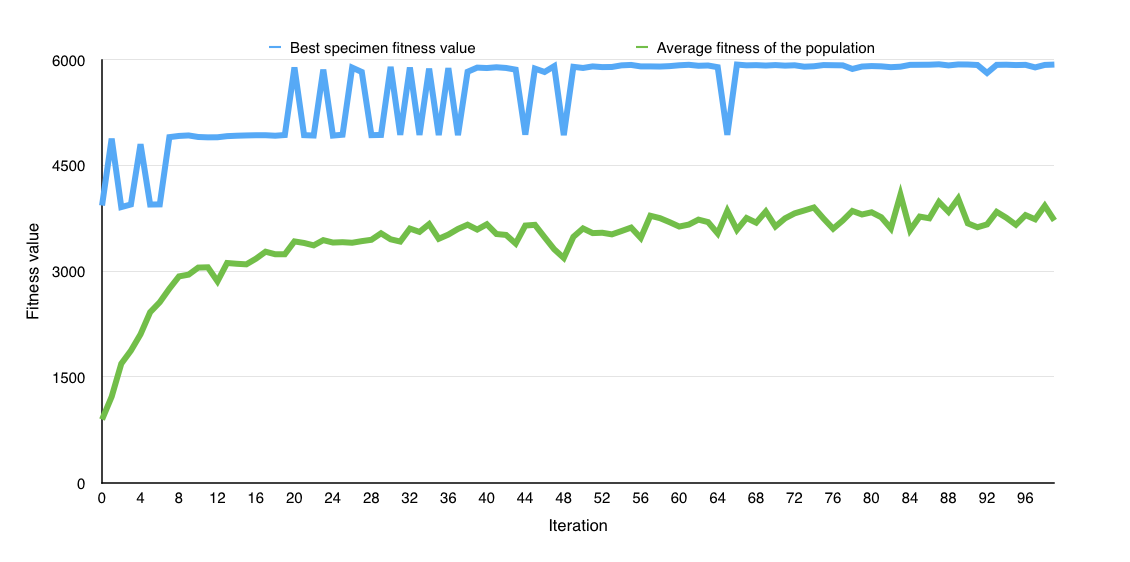
\includegraphics[scale=0.6]{competitivefitnessplot}
    \caption{A fitness value with respect to iteration plot in the competitive scenario.}
    \label{fig:x competitivefitnessplot}
\end{figure}

\begin{figure}[h]
    \centering
    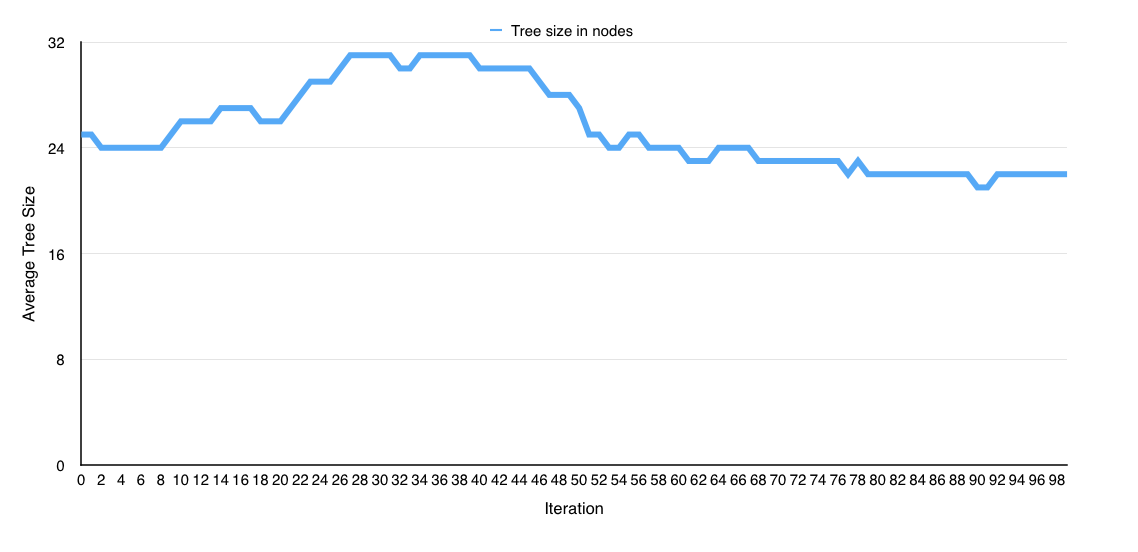
\includegraphics[scale=0.6]{competitivetreesizeplot}
    \caption{An average tree size with respect to iteration plot in the competitive scenario.}
    \label{fig:x competitivetreesizeplot}
\end{figure}
The algorithm's run in this particular case started on a relatively high note, with the best specimen claiming 4 markers for himself. In the next few iterations, best fitness achieved increased, then oscillated around 4200 value, to finally stabilize on a value closer to 5000. Up to this point, one can see the average fitness in the generation rising, indicating that, while there were no radical increases in value, the algorithm was producing more and more feasible candidates. Then, surely due to particularly good mutation or crossover operations, a breakthrough was made and the population achieved first successful specimen in the run. This one, however, was instantly lost, having not been copied over to the next generation. The curve then starts oscillating heavily, with the algorithm producing further successful specimen only to lose them few cycles later. Finally, around iteration 50 mark, the best specimen was kept for a longer duration. Note that the first successful individual marked the decline in average fitness growth, meaning that by that time, the population has been saturated with useful gene structures.

The size plot is intended to be considered and analyzed together with the fitness values. Having done that, one can observe that with the first successful specimen produced, the population started intensively increasing in node count. Having achieved large enough pool of fit solutions, size started to be the differentiating factor, successfully lowering the number. This is the perfect example of larger trees being promoted in the initial stages (since bigger trees have a higher chance of containing a useful node structure combination), but having their value decreased as the useful genes from them are passed into further generations. This also poses an balance question - whether the first found successful specimen should be accepted, or will processing more generations rewarding?

\begin{figure}[h]
    \centering
    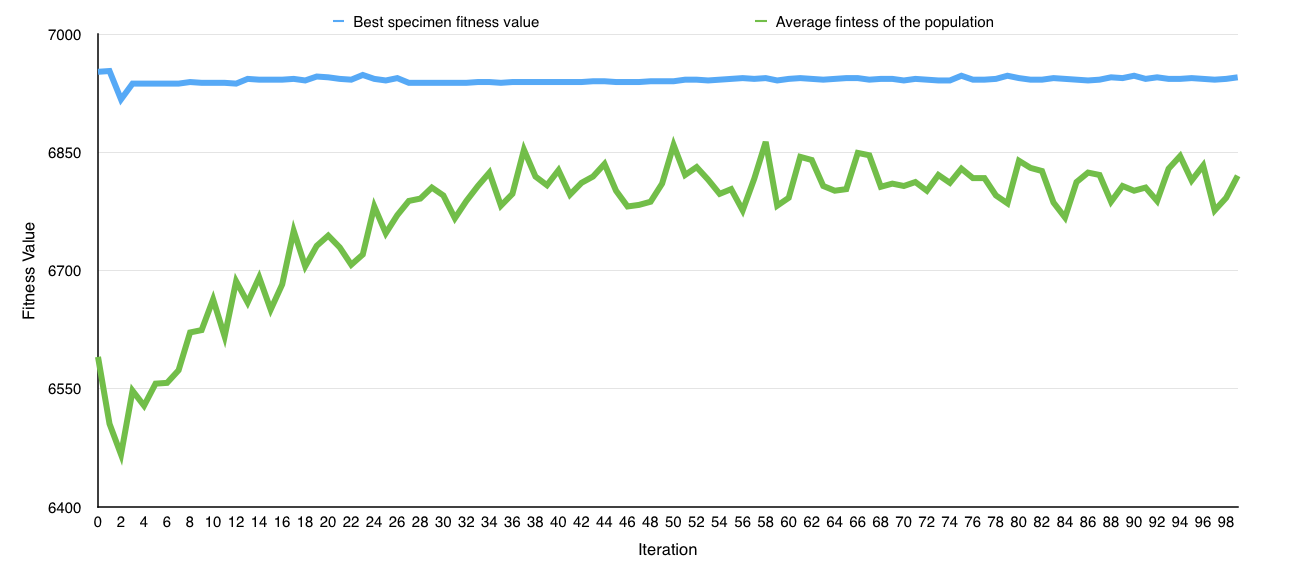
\includegraphics[scale=0.6]{cooperativefitnessplot}
    \caption{A fitness value with respect to iteration plot in the cooperative scenario.}
    \label{fig:x cooperativefitnessplot}
\end{figure}

\begin{figure}[h]
    \centering
    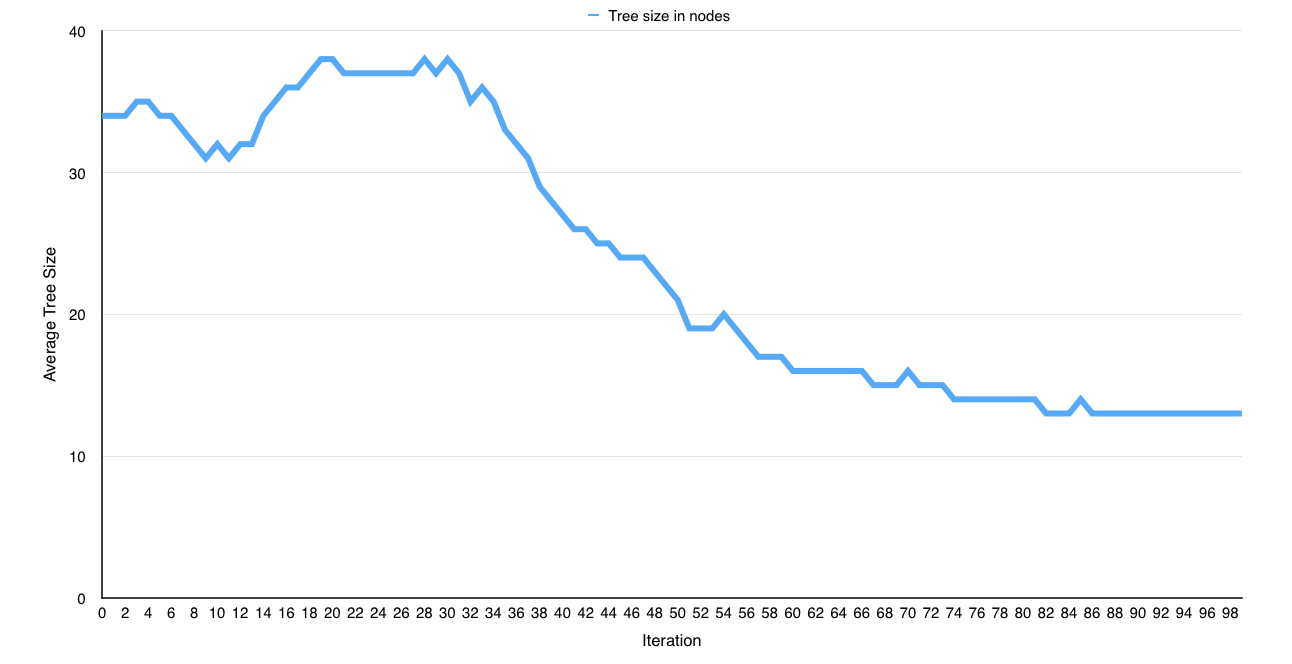
\includegraphics[scale=0.6]{cooperativetreesizeplot}
    \caption{An average tree size with respect to iteration plot in the cooperative scenario.}
    \label{fig:x cooperativetreesizeplot}
\end{figure}

Compared to the competitive scenario, the fitness plot in figure \ref{fig:x cooperativefitnessplot} presents much \textit{calmer} best fitness curve with no sudden changes in value, although with oscillations in abundance. Having produced a successful specimen in the first generation, the individual is instantly destroyed, its genes diluted in the pool of next generation. Another one, however, is produced as quickly as the fourth generation of the algorithm. The best specimen value starts oscillating with low amplitude, stabilizing after a good while. Average fitness value curve reflects that progress well, with the oscillations starting only when the other one stabilizes (again, marking the point where the population is saturated).

The progress of the population in the cooperative scenario is definitely more visible on figure \ref{fig:x cooperativetreesizeplot}. On 30th generation, when the fitness value of the best specimen appears to enter stagnation, abrupt decrease of an average specimen node count begins. Over the next 50 iterations of the algorithm, the average size is reduced almost thrice - from 36 nodes to 13.

While the average tree size of the population is an important indicator of the algorithm's overall health and progress (in a sense, since the progress can be presented as the ratio of current node count to the \textit{minimal solution} node count), it's the size of a best specimen tree that's important for the potential end-user. Figure \ref{fig:x competitivebestspecimentreesizeplot} presents the changing of the size of the best solution with regards to generation from one of the later experiments with increased tree size factor weight.

\begin{figure}[H]
    \centering
    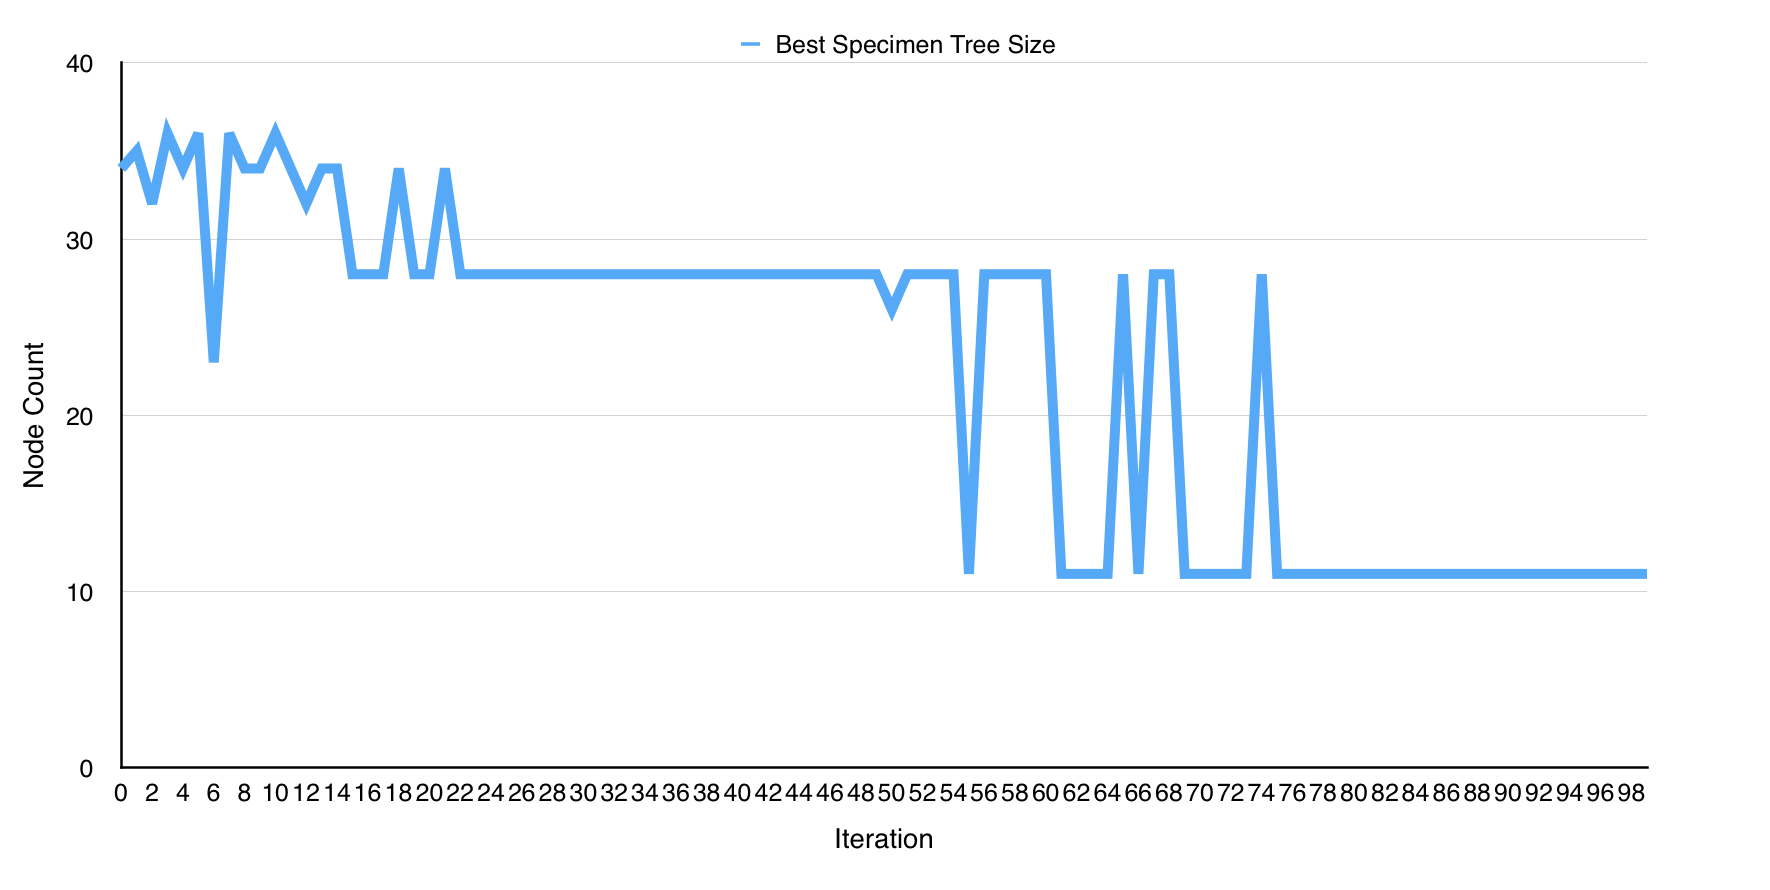
\includegraphics[scale=0.4]{bestspecimentreesizecomp}
    \caption{A best specimen tree size with respect to iteration plot in the competitive scenario.}
    \label{fig:x competitivebestspecimentreesizeplot}
\end{figure}

The relation between the size of the best specimen tree and the average tree size of the population can be compared to one between best specimen fitness value and average fitness of the population - the first few generations are a space for experiments, where size itself isn't more important than ever decreasing time. After coming up with a sufficiently big pool of good combinations of nodes, the decrease in size begins. 28 nodes is established as a size as early as 20th iteration, staying that way till generation 52, where the plateau is broken and, through a 20-generation oscillation cycle, new local optimum is reached.

Figure \ref{fig:x cooperativebestspecimentreesizeplot} presents identical changes, but experienced in cooperative scenario.
\begin{figure}[H]
    \centering
    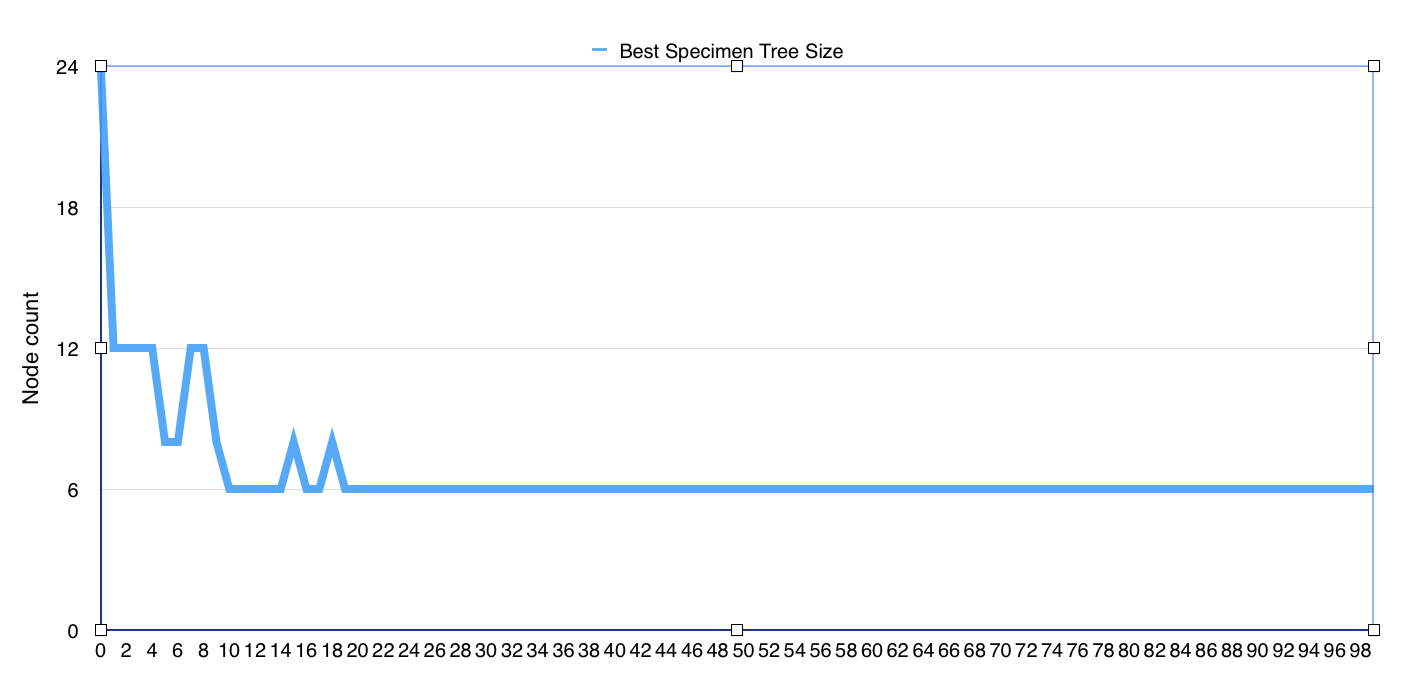
\includegraphics[scale=0.5]{bestspecimentreesizecoop}
    \caption{A best specimen tree size with respect to iteration plot in the cooperative scenario.}
    \label{fig:x cooperativebestspecimentreesizeplot}
\end{figure}
The decrease in node count in cooperative scenario is much more sudden - tree size had 10 times more influence on the fitness value of the specimen compared to competitive case (Table \ref{table:x tunedfitnessfunctionparameterscoop} for cooperative case, Table \ref{table:x tunedfitnessfunctionparameterscomp} for competitive case). With that large influence from the start, it is not unusual that the node count drops twice between the first and second generation. The decrease is sustained through the further generations (not without few slip-ups, when the best specimen was dropped from the population) to stabilize on 19th iteration.
\section{ Larger Scale Results } % this needs to change. Extended experiments?
To gain insight on how the algorithm's learning progresses through the two scenarios, we decided to compare the results of multiple executions. Given that the one full run of the algorithm takes 20 000 simulation runs, we decided it was necessary to distribute the testing over 10 computers, each capable of running two instances of our application at once without loss of performance. Given the resources available, we managed to achieve a large enough number of results in a reasonable amount of time.

Overall, we were able to gather 50 results per case. They were then analyzed using previously defined (in sections \ref{section_competitive_success} and \ref{section_cooperative_success}) criteria: in competitive scenario, successful specimen had to claim all possible markers; in cooperative case, candidate was deemed successful if his behavior improved on a total completion time. Tables \ref{table:x mass_results_comp} and \ref{table:x mass_results_coop} present a number of selected findings acquired in these experiments.

\begin{table} [H]
    \centering
    \begin{tabular} {l r}
        \hline \hline
        Description & Value \\
        \hline
        Successful specimen present after 10 generations & 18\% \\
        Successful specimen present after 50 generations & 70\% \\
        Successful specimen present after 100 generations & 78\% \\
        \\
        Minimum size achieved after 10 generations & 2\% \\
        Minimum size achieved after 50 generations & 18\% \\
        Minimum size achieved after 100 generations & 20\% \\
    \end{tabular}
    \caption{Selected facts from statistical data gathered from larger scale experiments in competitive case}
    \label{table:x mass_results_comp}
\end{table}

\begin{table} [H]
    \centering
    \begin{tabular} {l r}
        \hline \hline
        Description & Value \\
        \hline
        Successful specimen present after 10 generations & 20\% \\
        Successful specimen present after 50 generations & 40\% \\
        Successful specimen present after 100 generations & 50\% \\
        \\
        Minimum size achieved after 10 generations & 56\% \\
        Minimum size achieved after 50 generations & 70\% \\
        Minimum size achieved after 100 generations & 70\% \\
    \end{tabular}
    \caption{Selected facts from statistical data gathered from larger scale experiments in cooperative case}
    \label{table:x mass_results_coop}
\end{table}

The full results of the testing are visible on Figure \ref{fig:x mass_test_plots}, containing two plots depicting success ratio in the set of 50 results through the algorithm's iterations (Figure \ref{fig: massfitnesscomp} for competitive case, Figure \ref{fig: massfitnesscoop} for cooperative one), as well as two plots with the additional metric: Figures \ref{fig: masstreesizecomp} and \ref{fig: masstreesizecoop} present success rate of the algorithm producing specimen of a minimal accepted tree size: that number was picked separately for each scenario based on the previous notion of the solutions' design. Table \ref{table:x mass_test_success_criteria} contains all criteria used in determining success of the selected metrics.
\begin{figure}[H]
    \centering
    \begin{subfigure}[b]{0.4\textwidth}
        \centering
        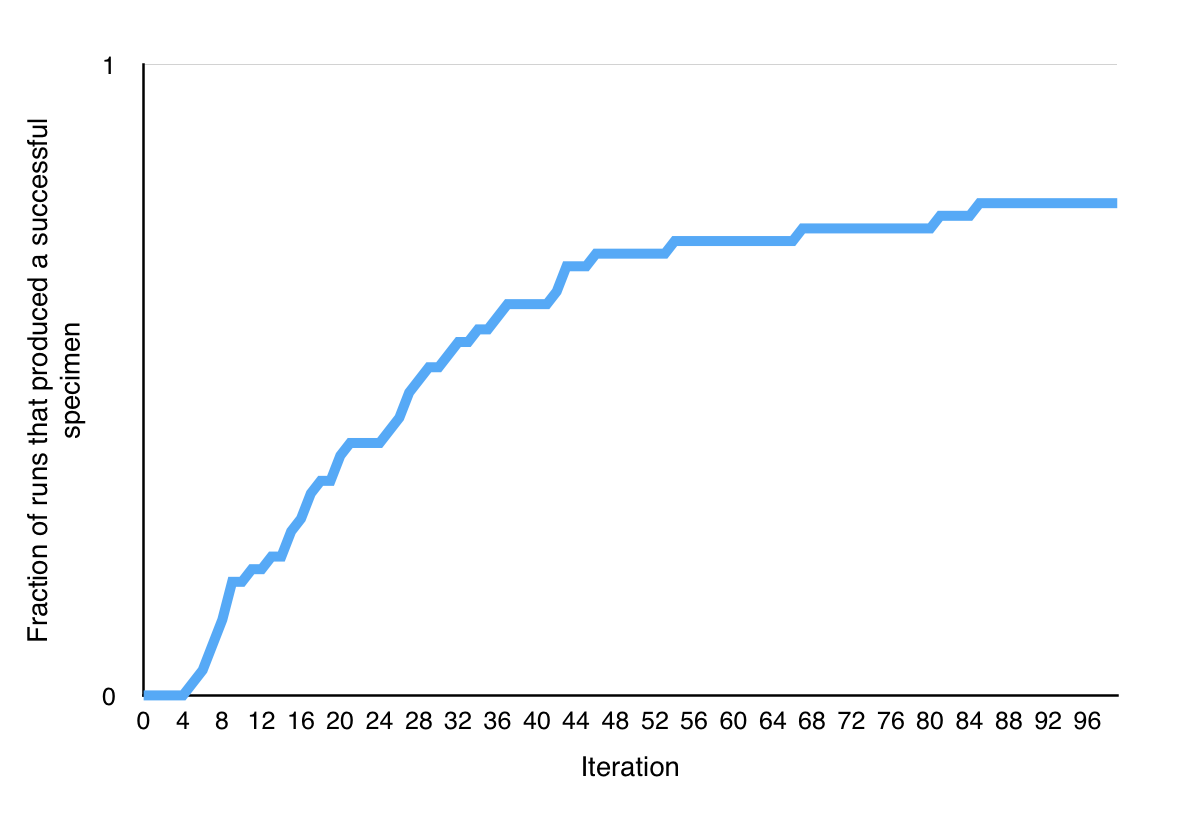
\includegraphics[width=\textwidth]{mass_test_fitness_comp}
        \caption{Success ratio progression with the number of iterations in competitive scenario}
        \label{fig: massfitnesscomp}
    \end{subfigure}
    \hfill
    \begin{subfigure}[b]{0.4\textwidth}
        \centering
        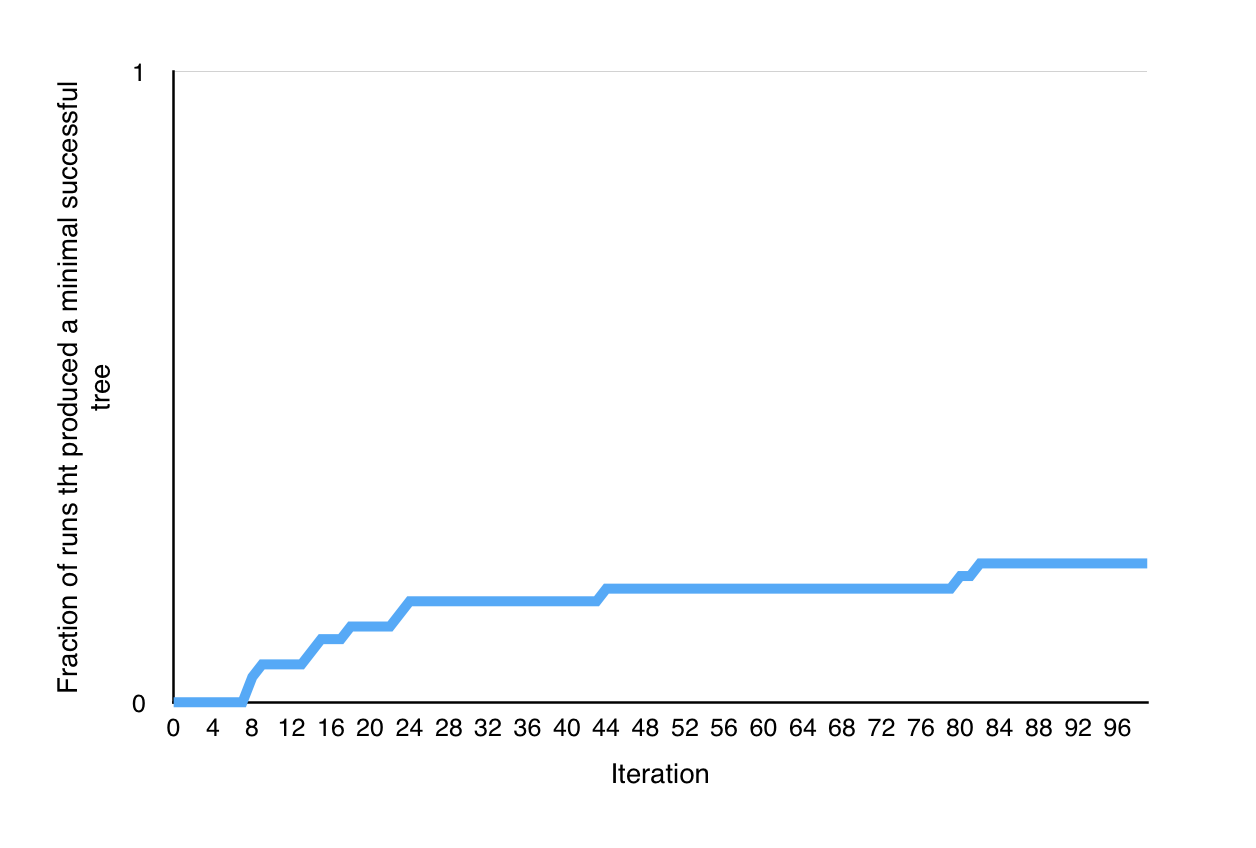
\includegraphics[width=\textwidth]{mass_test_treesize_comp}
        \caption{Minimal tree size acquirement ratio progression with the number of iterations in competitive scenario}
        \label{fig: masstreesizecomp}
    \end{subfigure}

    \begin{subfigure}[b]{0.4\textwidth}
        \centering
        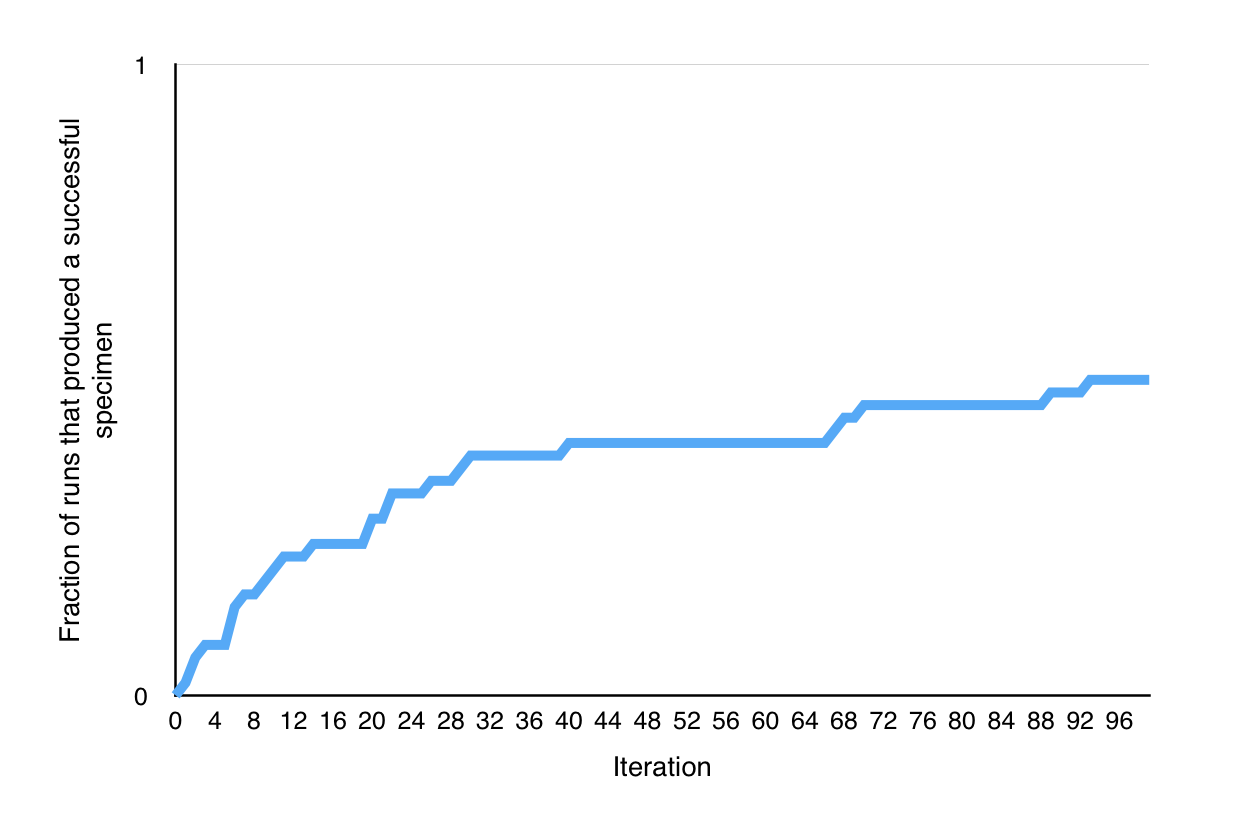
\includegraphics[width=\textwidth]{mass_test_fitness_coop}
        \caption{Success ratio progression with the number of iterations in cooperative scenario}
        \label{fig: massfitnesscoop}
    \end{subfigure}
    \hfill
    \begin{subfigure}[b]{0.4\textwidth}
        \centering
        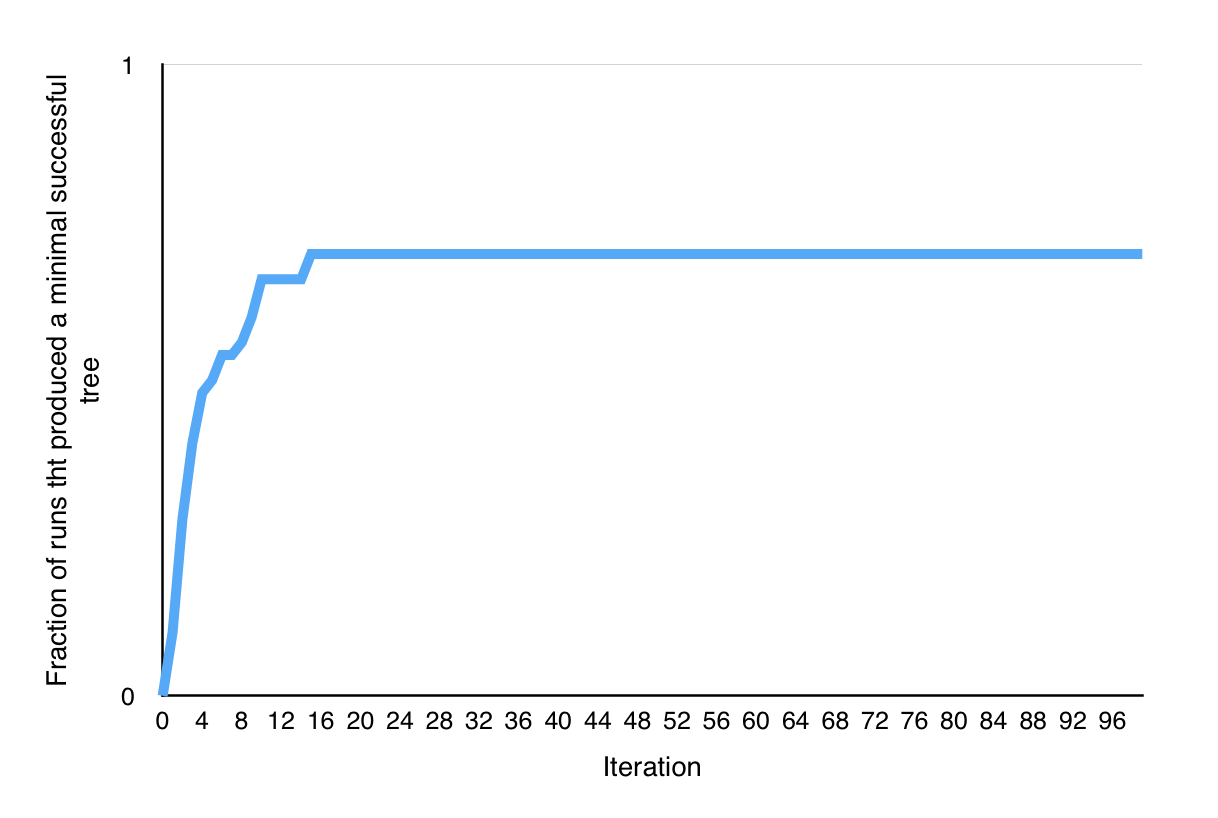
\includegraphics[width=\textwidth]{mass_test_treesize_coop}
        \caption{Minimal tree size acquirement ratio progression with the number of iterations in cooperative scenario}
        \label{fig: masstreesizecoop}
    \end{subfigure}
    \caption{Collected results of a larger scale experiments}
    \label{fig:x mass_test_plots}
\end{figure}

\begin{table} [H]
    \centering
    \begin{tabular} {l r}
        \hline \hline
        Criterion & Value \\
        \hline
        Minimum number markers claimed in competitive scenario & 6 \\
        Maximum size of a specimen allowed in competitive scenario & 7 \\
        Maximum time of completion allowed in cooperative scenario & 4.5s \\
        Maximum size of a specimen allowed in cooperative scenario & 4 \\
    \end{tabular}
    \caption{Criteria used in determining success ratio in experiments.}
    \label{table:x mass_test_success_criteria}
\end{table}

\newpage
The important thing to note when analyzing the results is the fact that the two scenarios' rates of success are not, directly or otherwise, comparable. Both Fitness and Tree Size \textit{goals} were chosen with great care, but remain only empirically picked values.
The overall success ratio, understood as ``percentage of algorithm's runs that produce at least one specimen that can be considered successful by $n-th$ generation'', underwent steady rise in both cooperative and competitive scenario, although two lengthy periods of stagnation can be observed during iterations 40-64 and 72-88 in cooperative case. While the growth rate itself will be discussed further down in this section, competitive case result greatly overshadowed cooperative scenario ratio, exhibiting much higher consistency.

Examining plots depicting minimizing of tree size progression, one can instantly see a difference in fitness function weighting, described previously in section \ref{section_fitness_function_tuning}. Adaptation in cooperative scenario is much more focused on size of the specimen, to the point where over our criterion for size was fulfilled by 10th generation in over 50\% of the results. Even so, 30\% of results didn't reach the requirement by 100th generation - almost certainly stuck in local minima. The situation in competitive scenario is quite different, however. The progression systematically rises through local plateaus, but the results at the and show that only 20\% of the results produced a specimen of a required size. Results from this variant, however, show a continuous improvement to the very end of testing; long period of stagnation observed in results of cooperative case after a rapid rise up to 15th generation are a clear indication that in 30\% of the cases, a larger rate of mutation would be needed to break the local optima.

Figures \ref{fig:x mass_test_two_scenarios} and \ref{fig:x mass_test_two_scenarios_normalized} were created in order to help with analysis of success ratio growth rate, that is to say the learning progression of the algorithm. Figure \ref{fig:x mass_test_two_scenarios} contains the two plots previously seen on figures \ref{fig: massfitnesscomp} and \ref{fig: massfitnesscoop} side by side. Figure \ref{fig:x mass_test_two_scenarios_normalized} contains the same two plots, but normalized, for the purposes of more direct comparison. The normalization was done with the assumption that both cases reached their respective global optima at the end of 102th generation - while this might be proven not to be the case, the comparison of the learning rate of the algorithm up to that moment is available to us at that moment.
\begin{figure}[h]
    \centering
    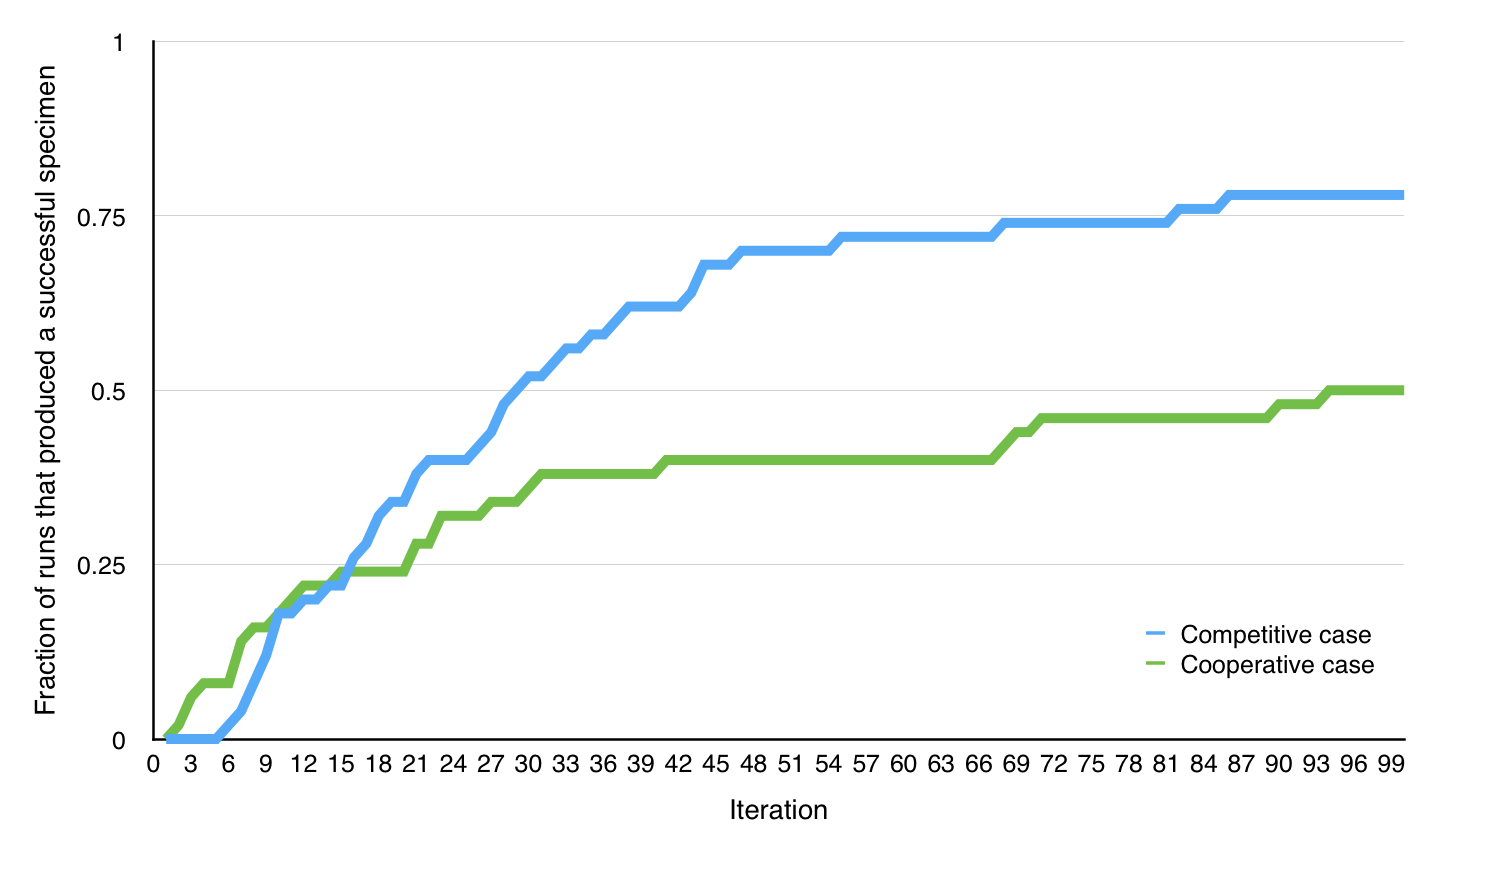
\includegraphics[scale=0.4]{mass_test_two_scenarios}
    \caption{Success ratio progression wit the number or iterations in competitive and cooperative scenarios}
    \label{fig:x mass_test_two_scenarios}
\end{figure}

\begin{figure}[h]
    \centering
    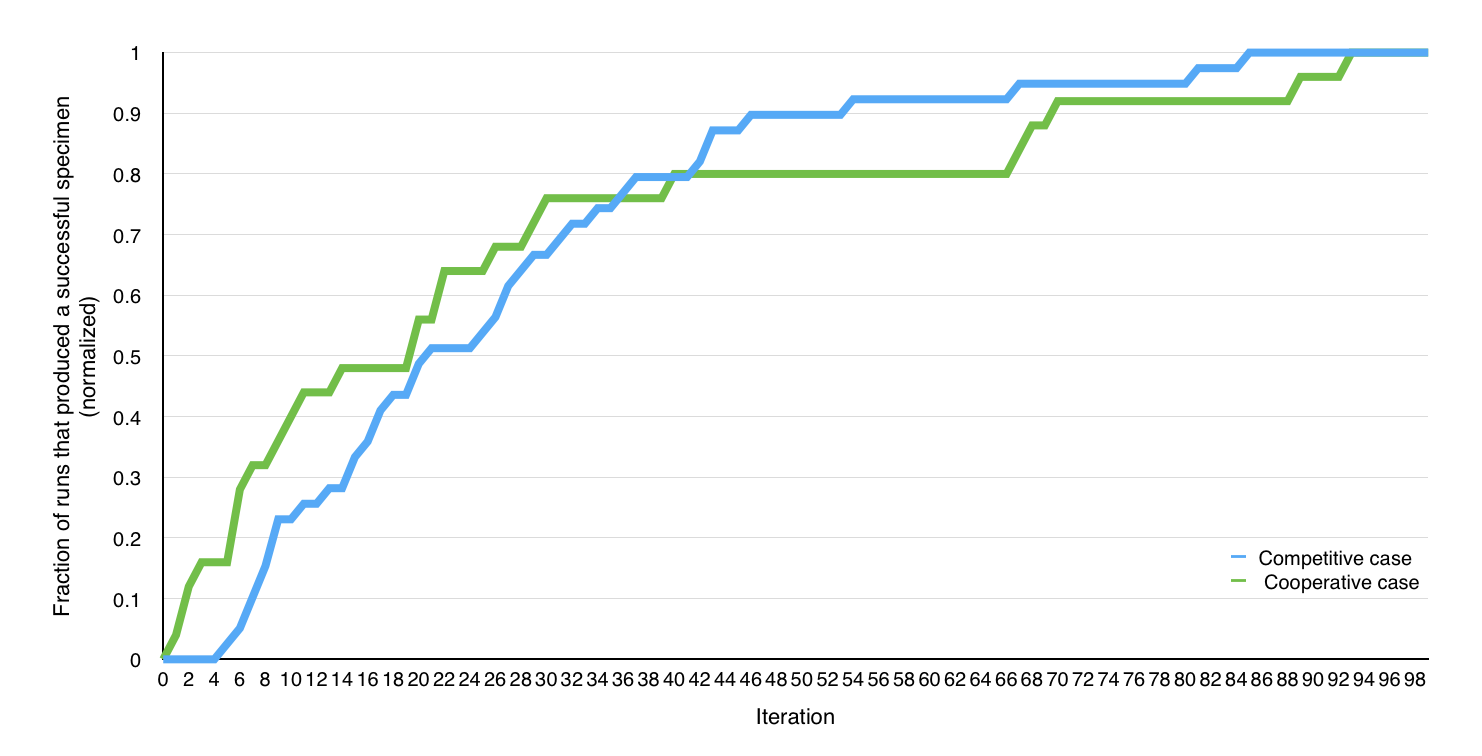
\includegraphics[scale=0.4]{mass_test_two_scenarios_normalized}
    \caption{Normalized success ratio progression wit the number or iterations in competitive and cooperative scenarios}
    \label{fig:x mass_test_two_scenarios_normalized}
\end{figure}

The two curves depicted next to each other testify to how similar the problems are when the learning progression is compared. The small advantage of the cooperative scenario curve displayed in iterations 0 to 38 stops at a point in which the two curves intersect - from this point onward, competitive scenario clearly grows in a higher rate. The intersection point from the perspective of cooperative case happens during a longer stagnation period, and then again, at the start of a next one. The growth of success rate was different between the two intersection points, with competitive results exhibiting 2 percent points less growth then cooperative did. At a point of cooperative case being overtaken it showed 38\% success rate, compared to 60\% yielded by competitive scenario. Unfortunately, without proper error measurement it's impossible to state with full certainty that this curve positioning, with cooperative case growing quicker at the beginning only to fall off in approximately one third of the experiments is, in fact, of significance.
